Deep learning (DL) models are used in multiple areas, ranging from e-mail spam filtering~\cite{blanzieri2008survey} in natural language processing (NLP) to image segmentation tasks for autonomous driving~\cite{he2017mask} in computer vision (CV).
The improvement of these models is not only based on more advanced architectures or algorithms~\cite{vinyals2015show, szegedy2015going, lai2015simultaneous}, but also on increased quality and quantity of training data~\cite{Krizhevsky:2012:ICD:2999134.2999257,deng2009imagenet,lin2014microsoft,everingham2011pascal,szegedy2015going}.
Having more training data usually proves to be beneficial to the model performance~\cite{banko2001scaling}.

\vspace{-0.3cm}
\begin{figure}[h]
    \centering
    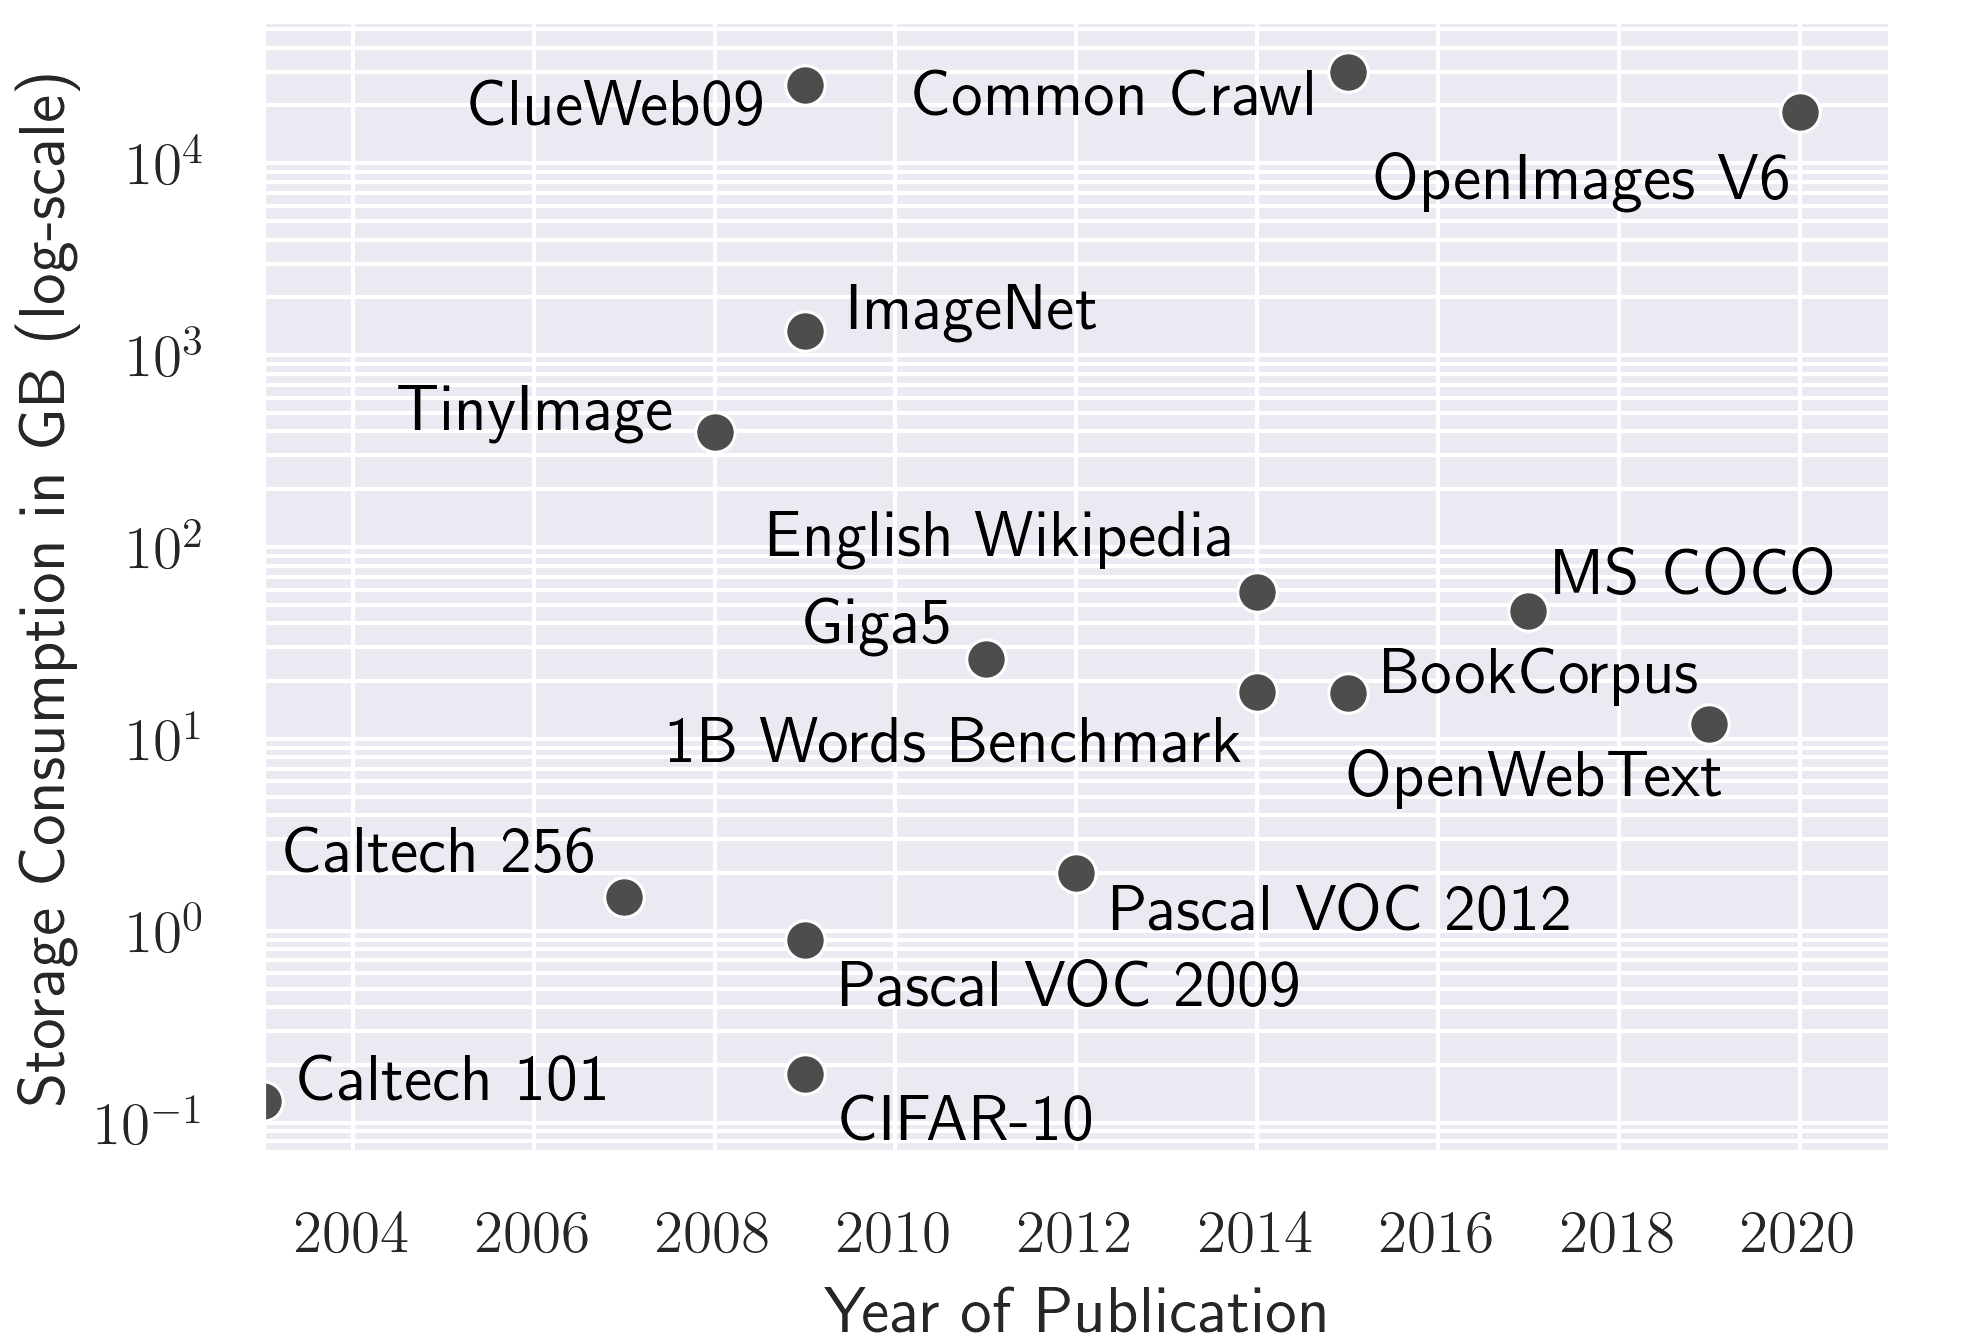
\includegraphics[width=0.47\textwidth]{figures/misc/all-datasets-size-cropped.png}
    \vspace{-0.3cm}
    \caption{Storage consumption of real-world CV and NLP datasets over time on a logarithmic scale. CV:~\cite{fei2004learning, griffin2007caltech, torralba200880, deng2009imagenet, pascal-voc-2009, everingham2011pascal, krizhevsky2009learning, lin2014microsoft, OpenImages2}, NLP:~\cite{callan2009clueweb09, giga5,chelba2013billion, engwiki, zhu2015aligning, commoncrawl, Gokaslan2019OpenWeb}.}
    \label{fig:all-datasets}
\end{figure}
\vspace{-0.2cm}

The process to train a DL model consists of repeatedly iterating over the entire training dataset, measuring up to hundreds of iterations depending on the task at hand and the model complexity~\cite{peters2018deep,he2016deep,szegedy2015rethinking,radford2018improving}.
Popular datasets show exponential storage consumption increase over time (Fig.~\ref{fig:all-datasets}), which makes data preprocessing harder, as local processing is not viable anymore due to memory limitations. Both distributed storage solutions~\cite{weil2006ceph} as well as distributed processing~\cite{gabriel2004open, vishnu2016distributed, beam,zaharia2010spark, 10.1145/3363554} can lead to new difficulties with network I/O and latency, which makes data preprocessing an integral part of the end-to-end DL pipeline.
A Google study on their cluster fleet showed that the preprocessing pipeline takes more than a third of the total preprocessing time for 20\% of their jobs~\cite{murray2021tf}.

Optimizing the model training is an active research topic that focuses on decreasing the total training time and increasing the data ingestion rate of the training process.
There are many methods on training performance optimization and model optimization for both single GPU~\cite{micikevicius2017mixed,vanholder2016efficient,han2015deep} and multi-GPU setups~\cite{jager2018parallelized,sergeev2018horovod,Jia2019,ren2019performance} which allow for horizontal scaling with more hardware~\cite{nvidiabenchmarks2020}.
Recent hardware innovations help with improved model performance (cf. Fig.~\ref{fig:gpu-resnet-throughput}).
Therefore, it is essential to optimize preprocessing pipelines to keep up with the training process speed.

The preprocessing part of a DL pipeline consists of multiple successive data transformation steps applied to the initial dataset until the final data representation matches the model input dimensions.
This transformation can be performed once before the training or in every iteration while the training is happening.
For example, CV pipelines from DL models that established new landmarks at their respective times~\cite{krizhevsky2012imagenet,zeiler2013visualizing,Simonyan15,he2016deep,szegedy2015rethinking} follow a common pattern of preprocessing steps: \textit{read} the image from a storage device, \textit{decode} it into an RGB matrix and \textit{resize} the image to fit the model input dimensions. 
These steps can be followed by data augmentation, e.g., \textit{pixel-centering}, \textit{random-cropping} or a \textit{rotation}, depending on the particular use-case.
Preprocessing the full dataset once before training is viable if one wants to avoid the processing overhead in every iteration.

However, the final data representation and the storage device can negatively affect the preprocessing throughput.
The training process's data ingestion can be throttled by I/O bottlenecks when loading the preprocessed data.
The storage consumption typically increases at later preprocessing steps, as the corresponding data representations often store data inefficiently to facilitate processing (e.g., JPG~\cite{wallace1992jpeg} vs. an RBG matrix).
This additional storage consumption can be a determining factor that slows down the final throughput. The file system, storage device, and the data loader from the DL framework may not be able to read the data fast enough (cf. Section~\ref{sec:analysis}).

We propose a new, more flexible way to look at DL preprocessing pipelines, where the decision for \textbf{each} preprocessing step to apply it \textit{once} or in \textit{every iteration} can be made freely based on quantifiable trade-offs.
Such quantification can be provided by profiling.

%\vspace{-1.2cm}
\begin{figure}[h]
    \centering
    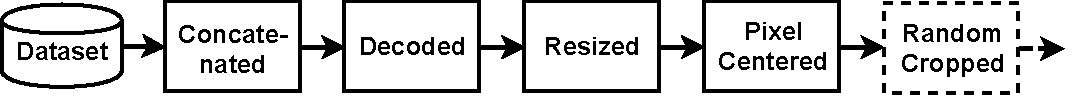
\includegraphics[width=0.47\textwidth]{figures/imagenet-pipeline/pipeline.pdf}
    \vspace*{-0.2cm}
    \caption{CV preprocessing pipeline}
    \label{fig:cv-pipeline}
\end{figure}
\vspace{-0.3cm}

To motivate this new view on preprocessing pipelines, we performed experiments using different configurations of a CV pipeline (Fig.~\ref{fig:cv-pipeline}){\color{diff} \footnote{The only step which has to be applied every iteration is \textit{random-crop}, as it is not deterministic (dotted line).}}.
{\color{diff} Performing all preprocessing steps \textit{at once} increases the throughput by $5.4\times$ compared to \textit{at every iteration} (Tab.~\ref{tab:intro:trade-offs-cv}).
However, this increases storage consumption by more than $10\times$.
In contrast, preprocessing the dataset \textit{once} just until the resize step results in a $16.7\times$ throughput increase while increasing the storage consumption only by $3.4\times$ compared to processing all steps at every iteration.}

\begin{table}[h]
\scalebox{0.73}{
\begin{tabular}{l|r|r}
\textbf{Preprocessing strategy}        & \textbf{Throughput in} $\frac{samples}{s}$ & \textbf{Storage Consumption in GB}     \\ \hline
all steps at \textit{every iteration}       & {\color{diff}107}                 & \textbf{146}                  \\ \hline
all steps \textit{once}                     & {\color{diff}576}                 & 1535                          \\ \hline
until \textit{resize} step, \textit{once}  & {\color{diff}\textbf{1789}}   & 494                           \\
\end{tabular}
}
\caption{Trade-offs for the CV pipeline at different preprocessing strategies.}
\label{tab:intro:trade-offs-cv}
\end{table}
\vspace{-0.5cm}

When comparing the data processing rate of a popular CV model, ResNet-50, to the different preprocessing strategies on state-of-the-art GPUs, we see that stalls on the A10, A30, and V100 can be prevented by using the optimal strategy (Fig. ~\ref{fig:gpu-resnet-throughput}).
In multi-node training setups and when using specialized hardware (TPUs), increasing preprocessing throughput demands becomes even more evident.

The idea of opening up the preprocessing pipeline and the resulting trade-offs have not been explored yet in a comprehensive fashion.
This void prevents ML practitioners from optimizing their end-to-end DL pipelines.
They lack guidance in how to do that, as well as tooling support to automate such optimizations.

\vspace{-0.5cm}
\begin{figure}[h]
    \centering
    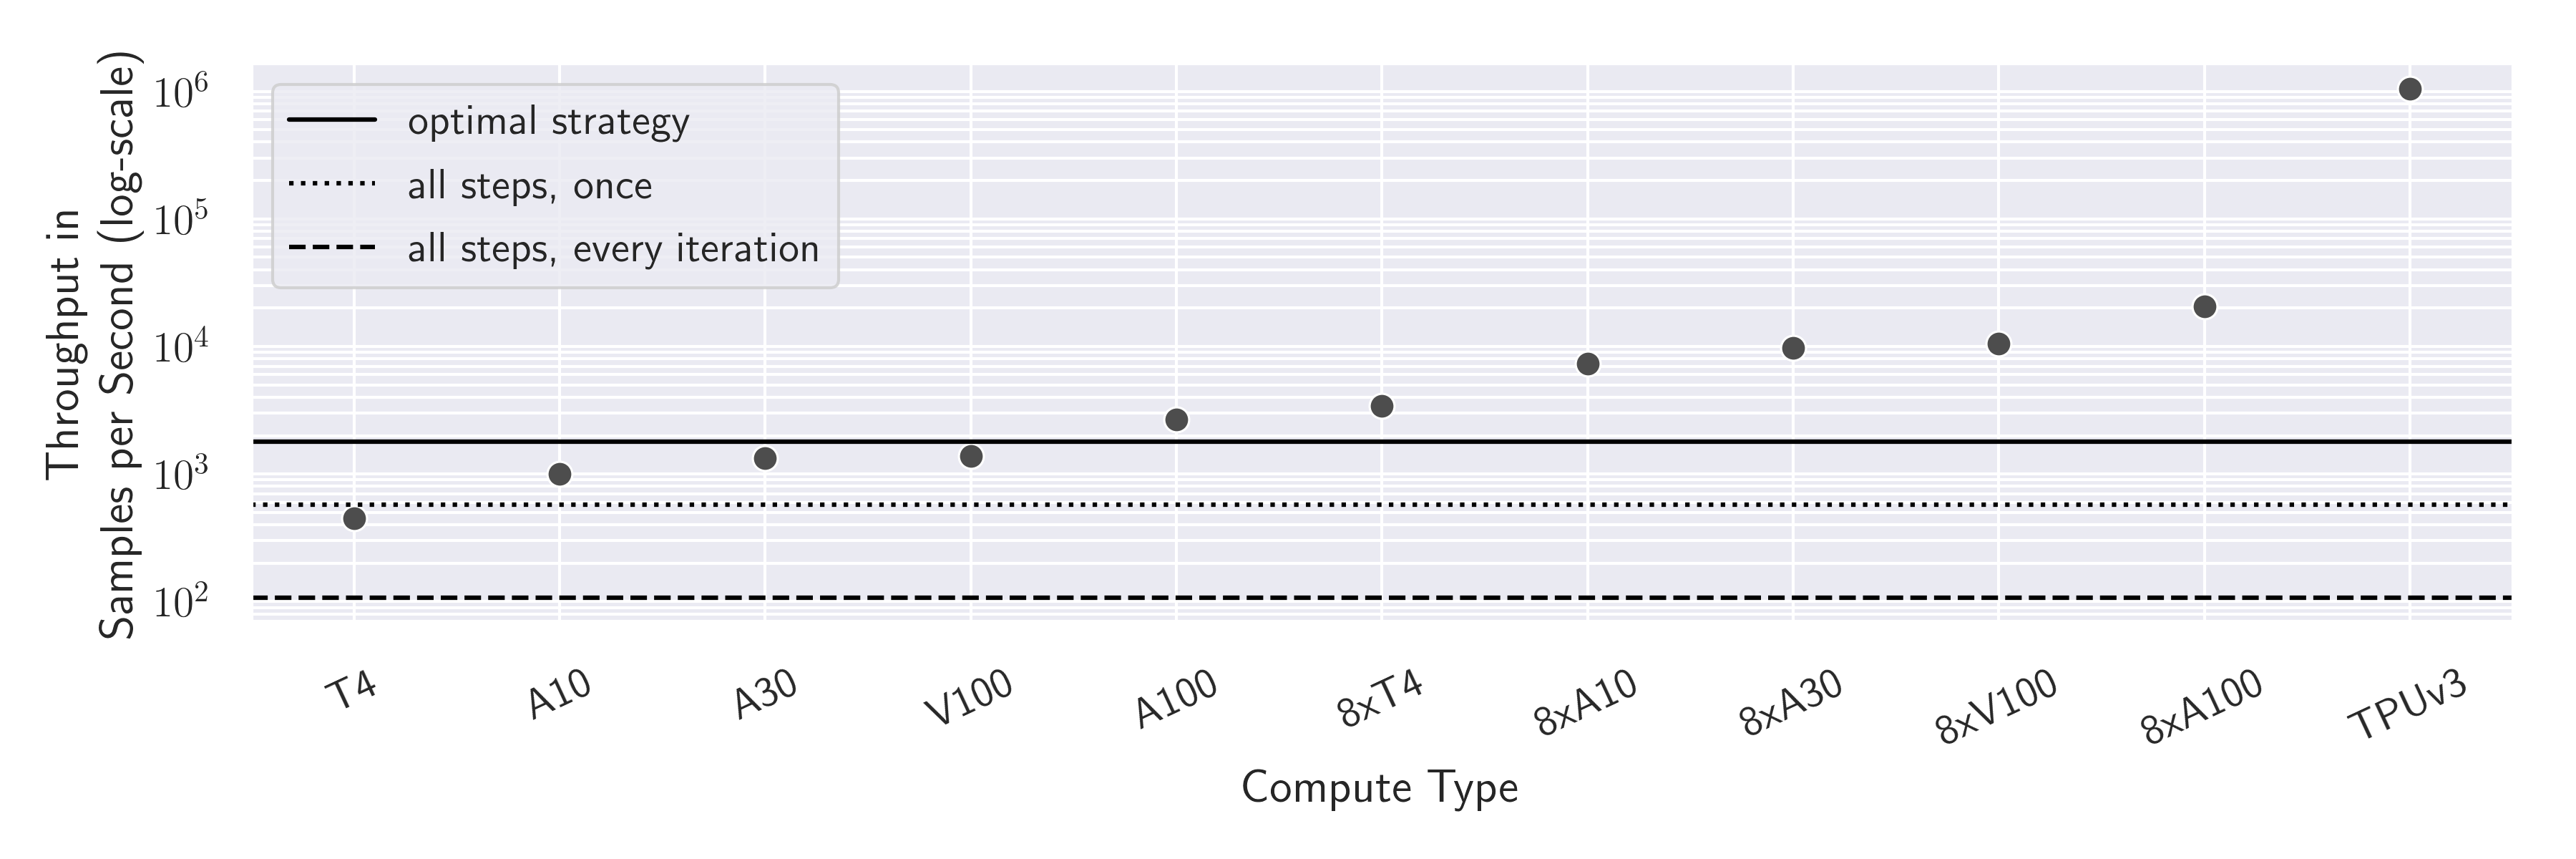
\includegraphics[width=0.48\textwidth]{figures/misc/gpu-comparison-resnet.png}
    \vspace{-0.8cm}
    \caption{Throughput of ResNet-50~\cite{he2016deep} for different hardware configurations. Black lines show the preprocessing throughput for the different strategies from Tab.~\ref{tab:intro:trade-offs-cv}. GPU profiling data from NVIDIA~\cite{nvidiabenchmarks2020} and TPUv3 by Ying et al.~\cite{ying2018image}.}
    \label{fig:gpu-resnet-throughput}
\end{figure}
\vspace{-0.4cm}

In this paper, we close this research gap by performing a comprehensive analysis of preprocessing pipelines from a broad range of different ML domains.
In doing so, we present practical insights into the pipelines themselves as well as the methodologies to analyze bottlenecks and an automated tool to perform profiling of arbitrary pipelines.
This opens up a new dimension in end-to-end ML system optimizations, which was not considered in prior works that targeted the pipeline optimization with respect to the model accuracy~\cite{mohan2020analyzing, kang2020jointly}.

Our contributions are:
\begin{enumerate}
    \item \textbf{We profile seven different real-world pipelines} and define the trade-offs and characteristics that allow practitioners to improve existing pipelines by optimizing at the location with the greatest impact on the training throughput. This way, we could improve training throughput by up to {\color{diff}3-13$\times$ compared to fully preprocessing once.}
    \item We provide lessons learned, where we \textbf{summarize the problems and unexpected findings} we encountered that can limit pipeline throughput. For example, we found that storage consumption {\color{diff}can affect the throughput negatively in different ways.} These insights can be used to clear up common misconceptions, and practitioners can be more aware of the impact the preprocessing pipeline has on the training performance.
    \item We present an open-source \textbf{profiling library} that automates the decision of which preprocessing strategy to pick based on a user-defined cost model.
\end{enumerate}

Our paper is organized as follows.
In Section~\ref{sec:preprocessing}, we introduce a general model and terminology of preprocessing pipelines.
The experimental setup and the library design are explained in Section~\ref{sec:experiments}.
We present our pipeline analysis and our findings in Section~\ref{sec:analysis}.
Our derived insights are summarized in Section~\ref{sec:lessons-learned}.
Related work is reviewed in Section~\ref{sec:related-work}.
Other approaches for pipeline optimizations are discussed in Section~\ref{sec:discussion} and we conclude the paper in Section~\ref{sec:conclusion}.